\newpage

\section{Induction Variables and Strength Reduction}
Strength reduction is an optimization technique which substitutes expensive operations with computationally cheaper ones. For example, a very weak strength reduction algorithm can substitute the instruction 
\texttt{b = a * 4} with \texttt{b = a << 2}.

\subsection{Motivation}

Opportunities for strength reduction arise routinely from details that the compiler
inserts to implement source-level abstractions. To see this, consider the simple
code fragment shown in Figure \ref{fig:p74-76}. Figure \ref{fig:p74} shows source code and the same loop in a low-level intermediate code.
 Notice the instruction sequence that begins at the label L2. The compiler inserted this code
(with its multiply) as the expansion of A[i]. Figure \ref{fig:p75}  shows the code that results from applying Strength Reduction,
Figure \ref{fig:p76} is followed by dead-code elimination. The compiler created a new variable, t2$^\prime$, to
hold the value of the expression i $*$ 4 + A. Its value is computed directly, by
incrementing it with the constant 4, rather than recomputing it on each iteration
as a function of i. Strength reduction automates this transformation. 

\begin{figure}[H]
    \centering
    \begin{subfigure}{0.6\textwidth}
    \centering
        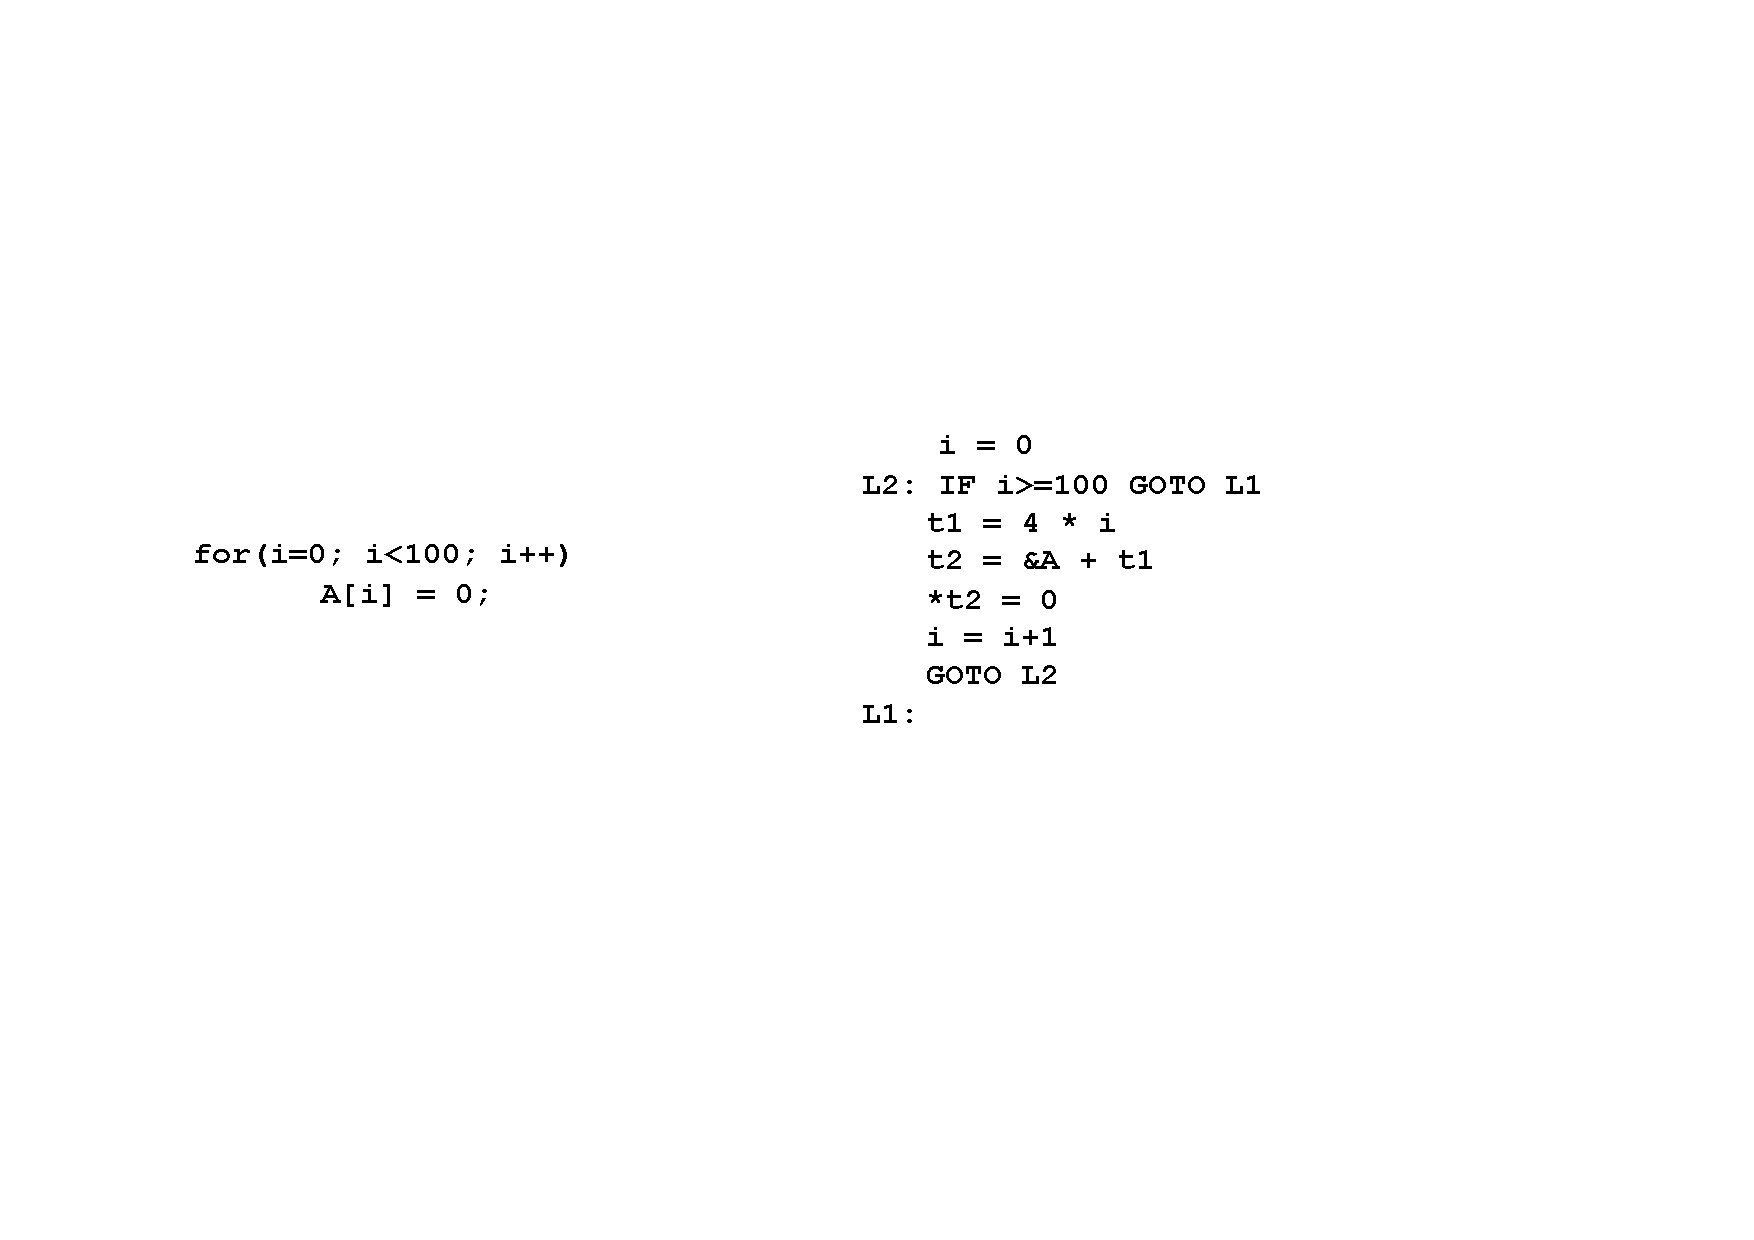
\includegraphics[width=\textwidth]{p74.pdf}
        \caption{Origianl code.}
        \label{fig:p74}
    \end{subfigure}
    \begin{subfigure}{0.6\textwidth}
    \centering
        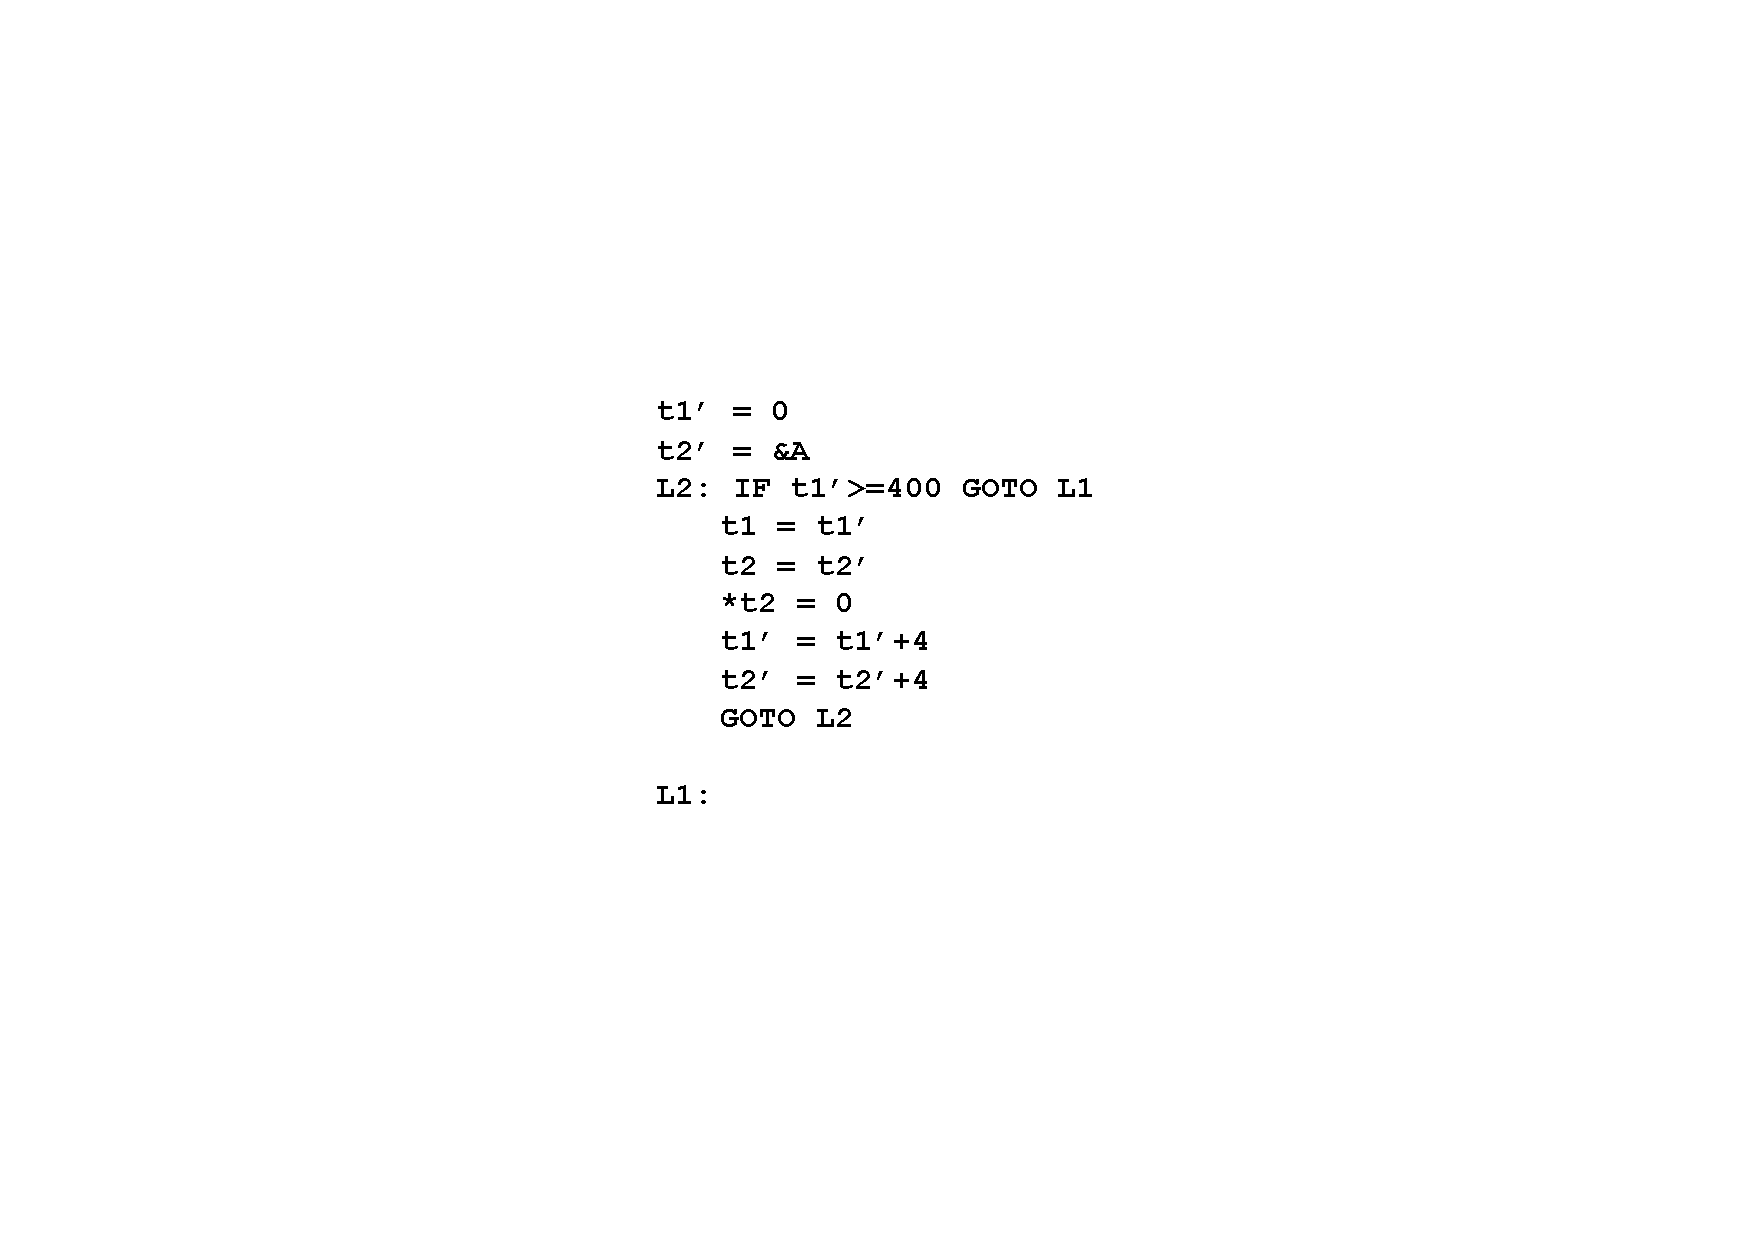
\includegraphics[width=\textwidth]{p75.pdf}
        \caption{After induction variable substitute.}
        \label{fig:p75}
    \end{subfigure}
    \begin{subfigure}{0.6\textwidth}
        \centering
            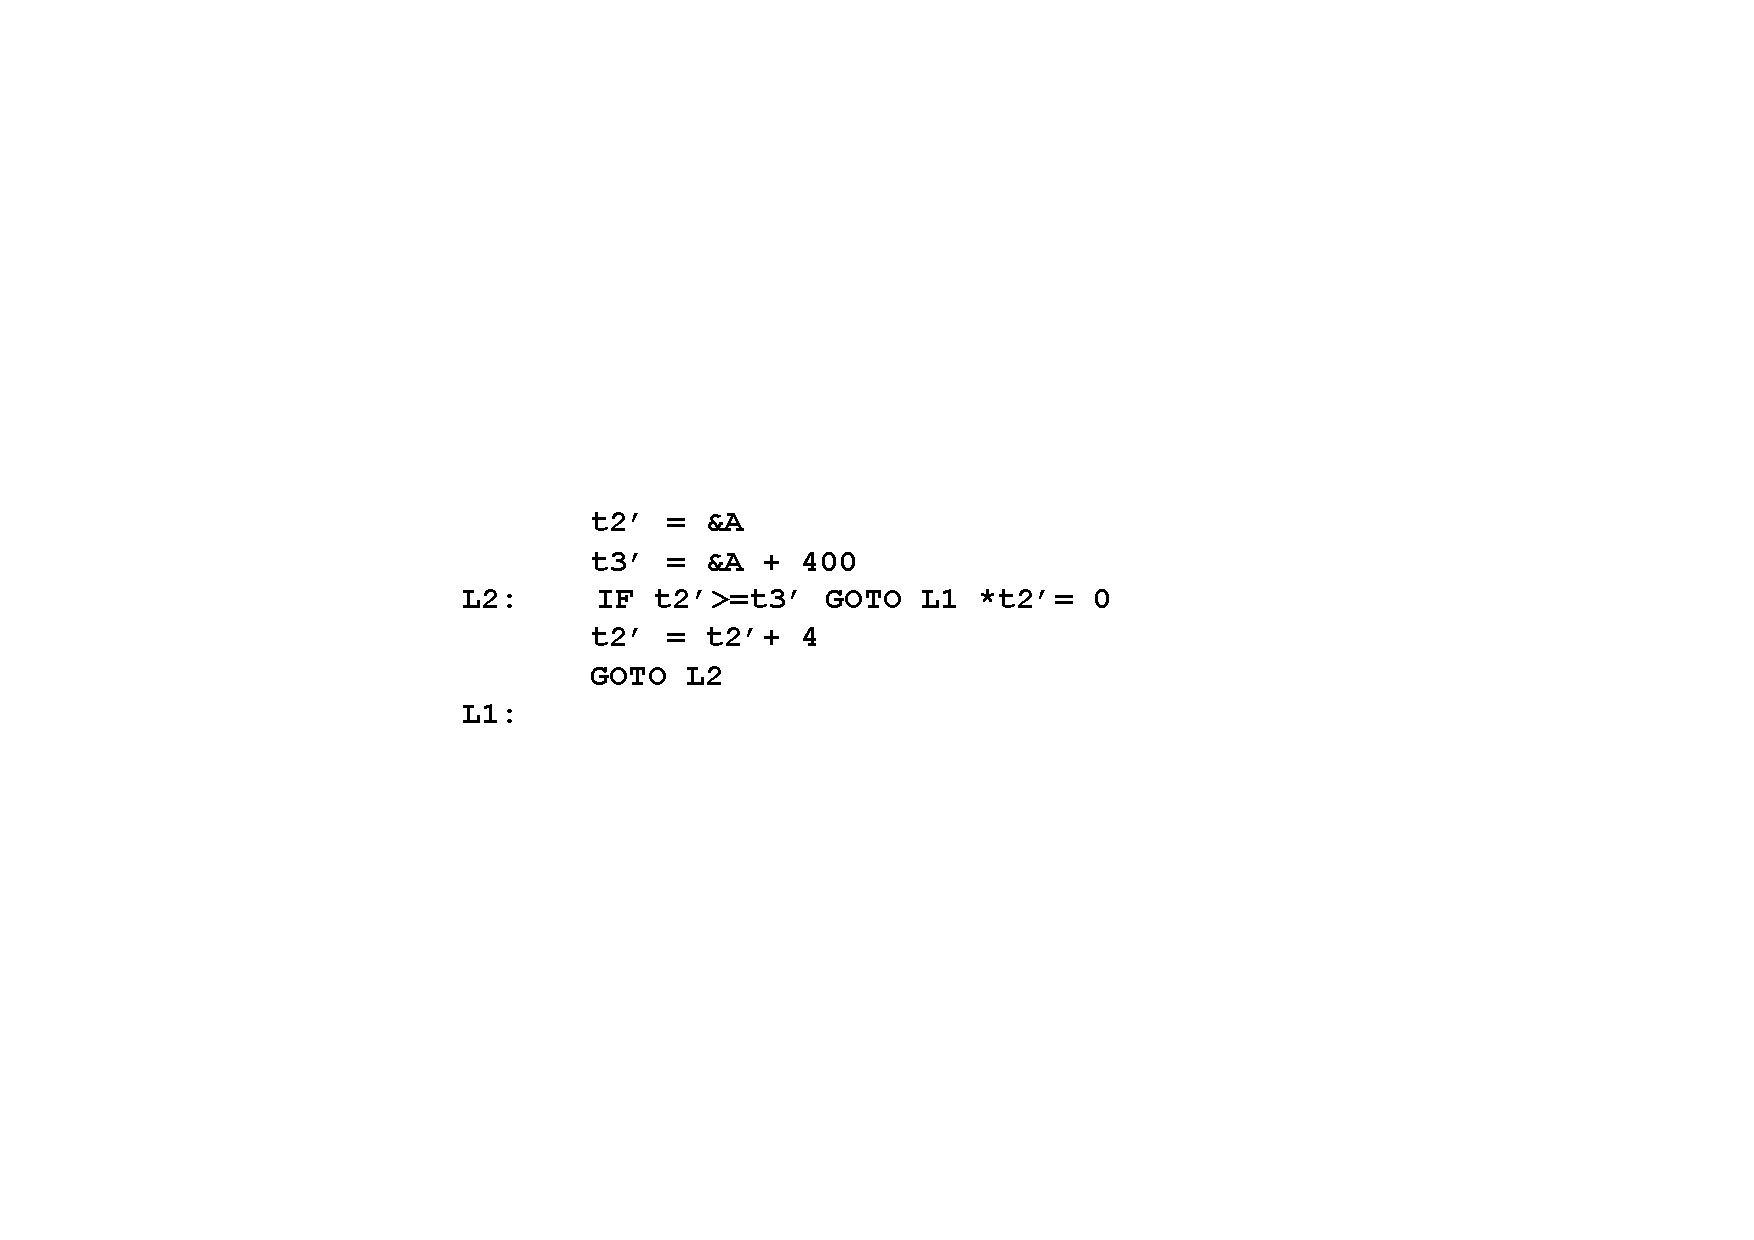
\includegraphics[width=\textwidth]{p76.pdf}
            \caption{Final code.}
            \label{fig:p76}
        \end{subfigure}
    \caption{An example of strength reduction.}
       \label{fig:p74-76}
\end{figure}



\subsection{Definitions}

\begin{definition}{Basic Induction Variable}
    A basic induction variable (e.g., i as shown in Figure \ref{fig:p74} ) is a variable X whose only definitions within the loop
are assignments of the form: X = X+c or X = X-c, where c is either a constant or 
a loop-invariant variable. 
\end{definition}

\begin{definition}{Induction Variable}
    An induction variable is either a basic induction variable B, or
or a variable defined once within the loop (e.g., t1,t2 as shown in Figure \ref{fig:p74} ) , whose value is a linear function
of some basic induction variable at the time of the definition:
$A = c_1 * B + c_2$
\end{definition}

The FAMILY of a basic induction variable B is the set of induction variables A such that each time A is assigned in the loop,
the value of A is a linear function of B. (e.g., t1, t2 is in family of i as shown in Figure \ref{fig:p74})


\subsection{Optimizations}

\subsubsection{Strength Reduction}
\begin{algorithm}[H]
    \caption{Strength Reduction Optimizations}\label{alg:Strength Reduction Optimizations}
    \begin{algorithmic}


    \State{A is an induction variable in family of basic induction variable B (i.e., $A = c_1 * B + c_2$ )}
    \State{\,\,\,\,\,\,\,\, Create new variable A$^\prime$}
    \State{\,\,\,\,\,\,\,\, Initialize in preheader A$^\prime$ = $c_1 * B + c_2$}
    \State{\,\,\,\,\,\,\,\, Track value of B: add after $B=B+x$: $A^\prime=A^\prime+x*c_1$}
    \State{\,\,\,\,\,\,\,\, Replace assignment to A: replace lone $A=\dots$ with $A=A^\prime$}
    \end{algorithmic}
    \end{algorithm}

\subsubsection{Optimizing non-basic induction variables}


\begin{itemize}
\item copy propagation
\item dead code elimination
\end{itemize}


\subsubsection{Optimizing basic induction variables}

Eliminate basic induction variables used only for calculating other induction variables and loop tests.   
\begin{algorithm}[H]
    \caption{Optimizing basic induction variables}\label{alg:Optimizing basic induction variables}
    \begin{algorithmic}


    \State{Select an induction variable A in the family of B, preferably with simple constants ($A = c_1 * B + c_2$ ).}
    \State{Replace a comparison such as \texttt{if B > X goto L1} with \texttt{if (A$\prime$ > $c_1 * X + c_2$) goto L1} (assuming c 1 is positive)}
    \State{if B is live at any exit from the loop, recompute it from A$\prime$, After the exit, $B = (A^\prime - c 2 ) / c 1$}
    \end{algorithmic}
    \end{algorithm}

\subsection{Further Details}


\begin{figure}[H]
    \centering
    \begin{subfigure}{0.7\textwidth}
    \centering
        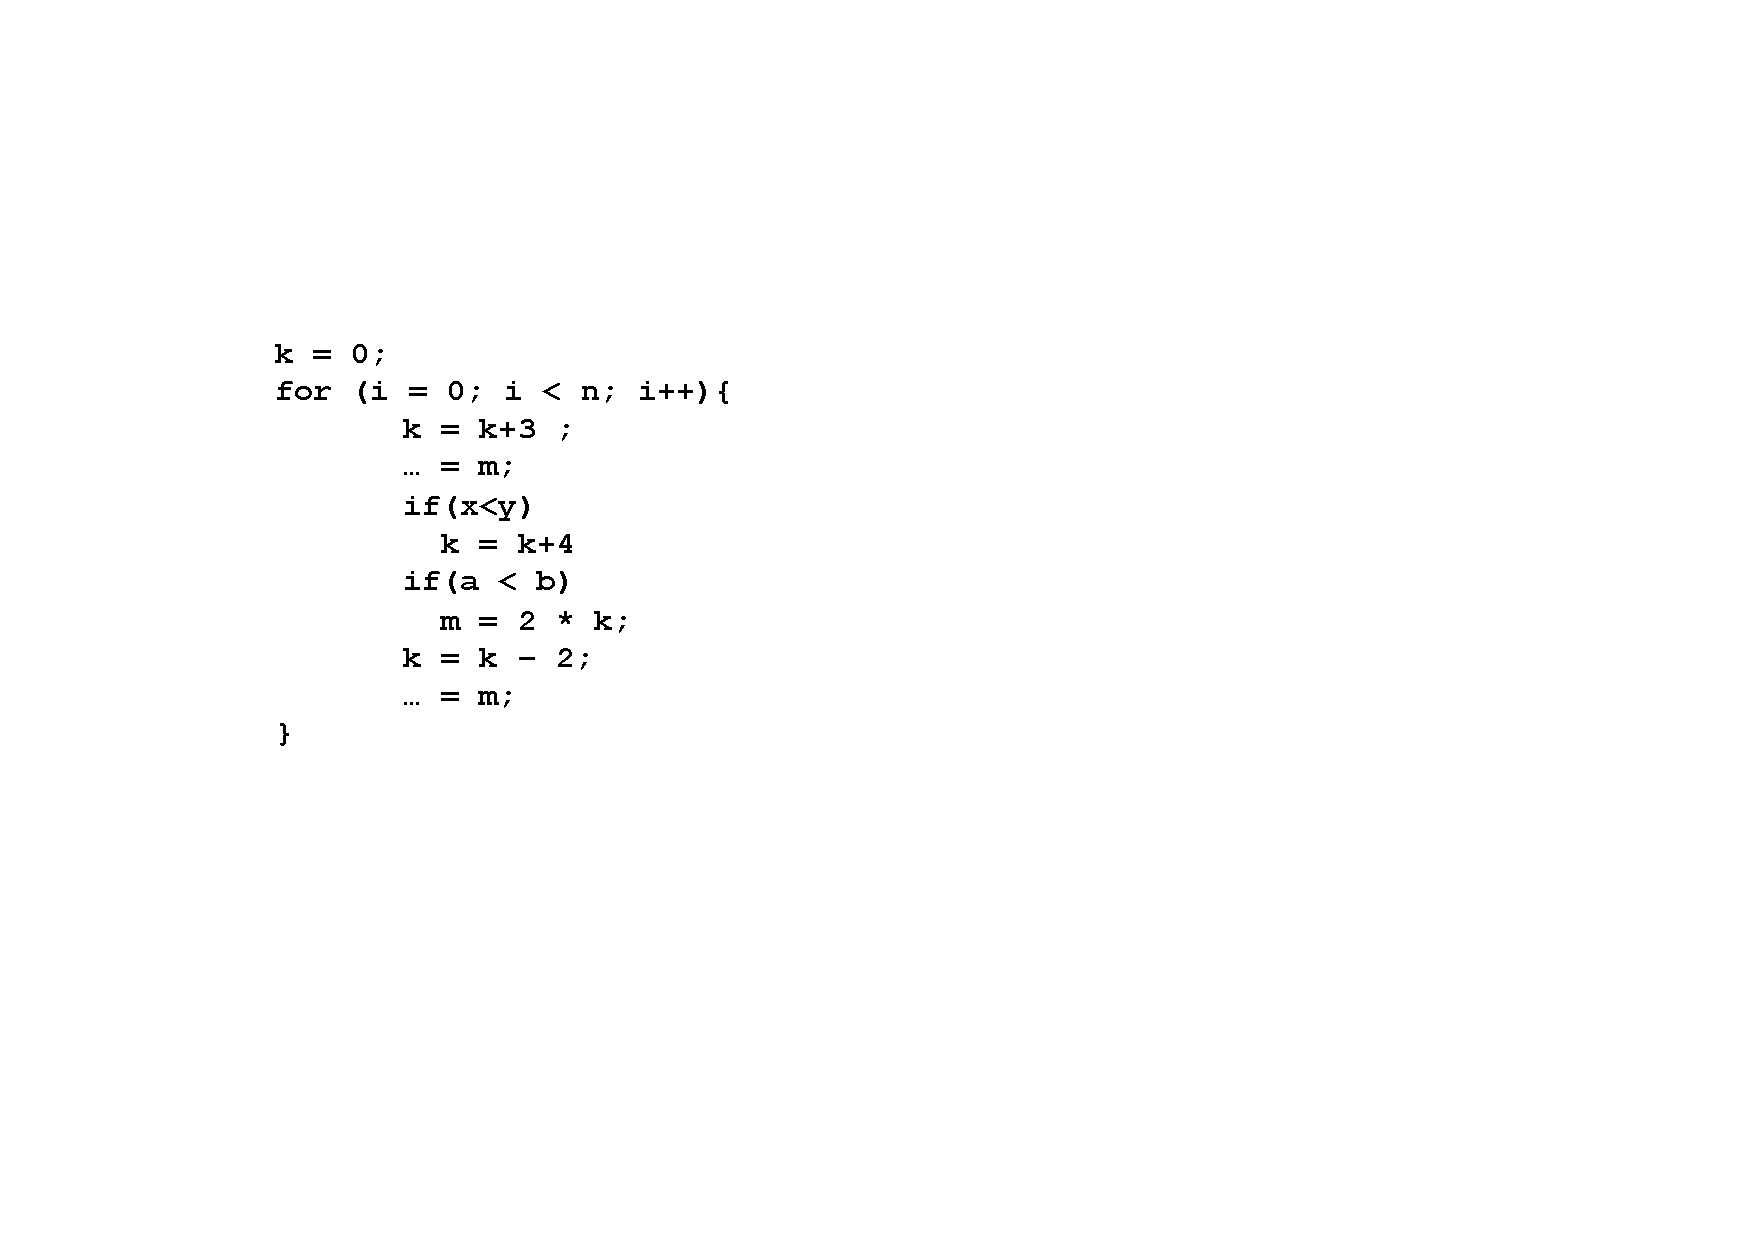
\includegraphics[width=\textwidth]{p78.pdf}
        \caption{A more complex example. k and i are both basic induction variables.
         m is in the family of k.}
        \label{fig:p78}
    \end{subfigure}
    \begin{subfigure}{\textwidth}
    \centering
        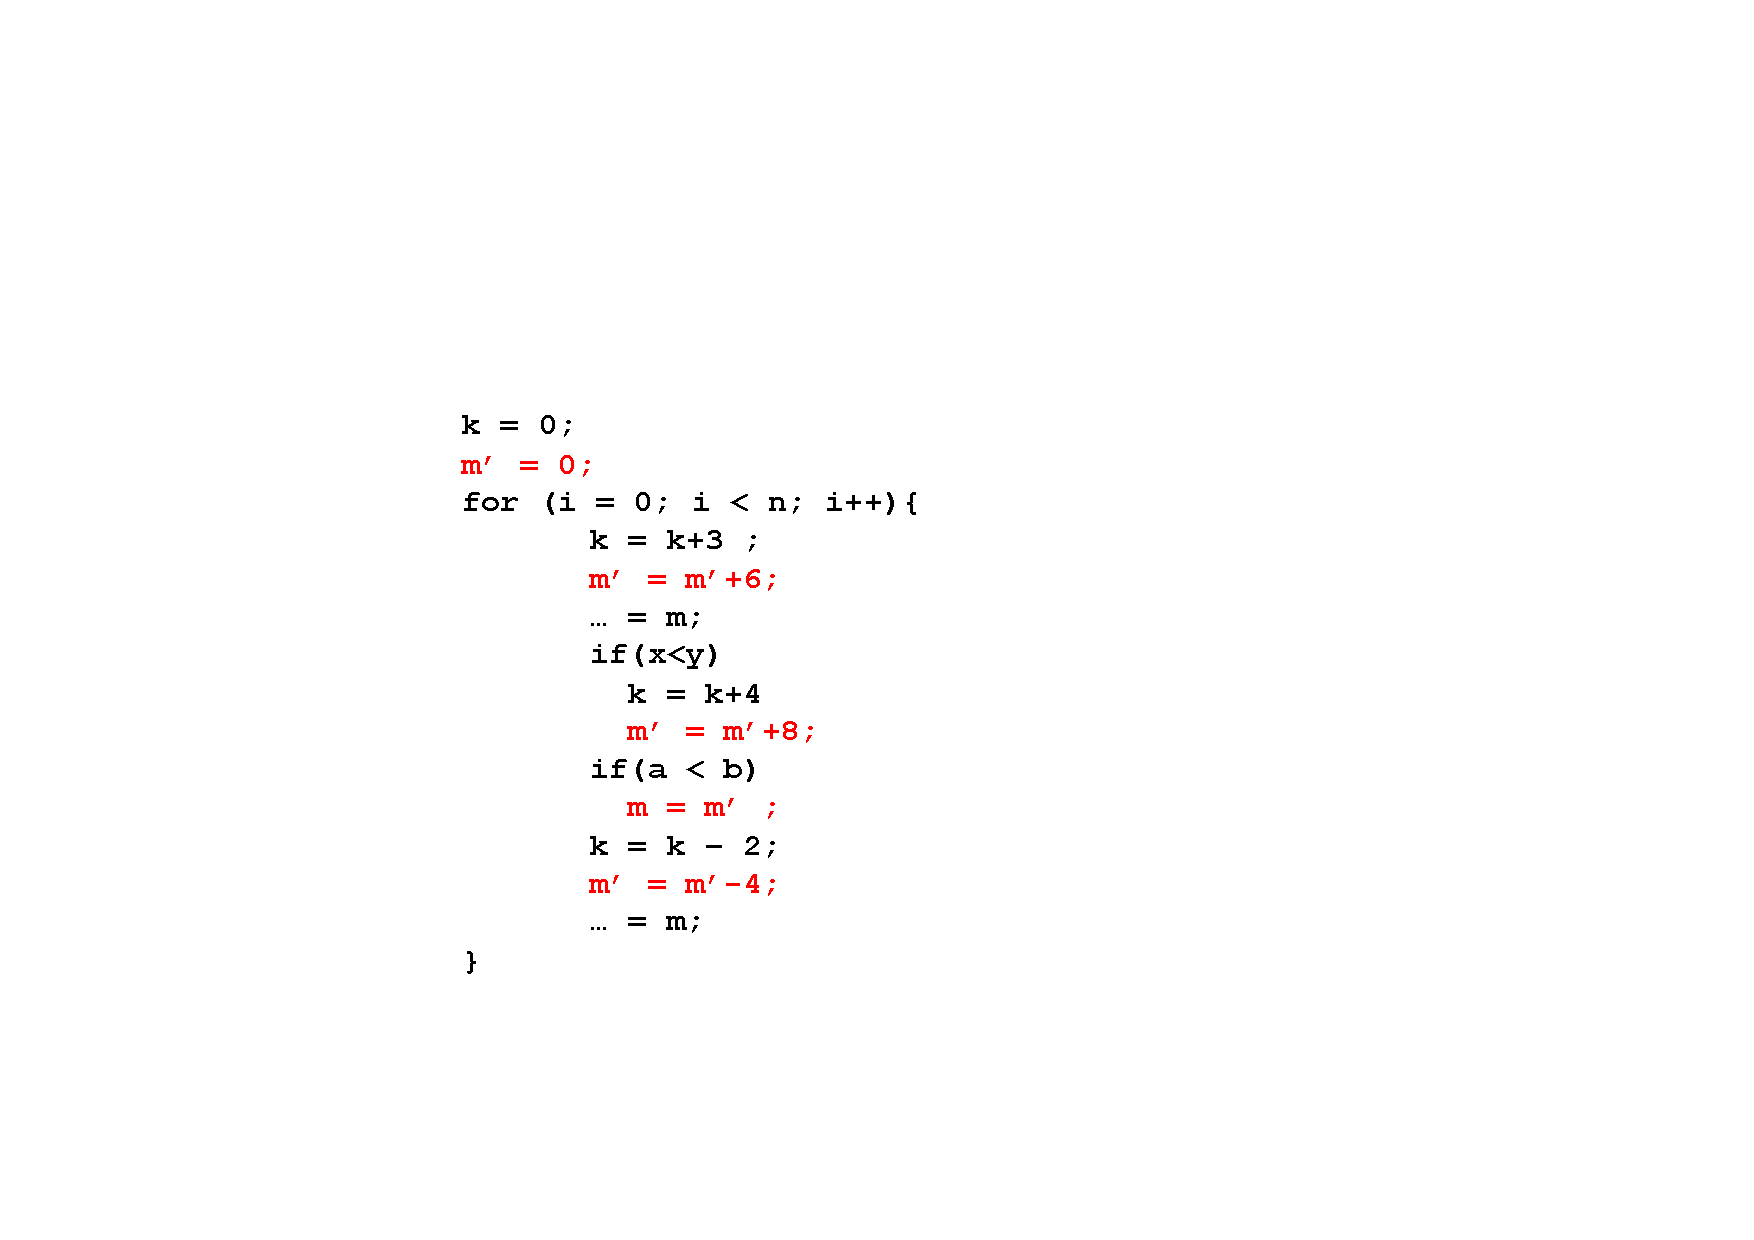
\includegraphics[width=0.7\textwidth]{p79.pdf}
        \caption{After induction variable substitute.}
        \label{fig:p79}
    \end{subfigure}
    
    \caption{A more complex example of strength reduction.}
       \label{fig:p74-76}
\end{figure}

\subsection{Finding Induction Variable Families}

Let B be a basic induction variable, A is in the family of B if it satisfies one the following conditions
\begin{itemize}
\item {\large{\textbf{Condition C1}}} A has a single assignment in the loop L of the form A = B*c, c*B, B+c, etc
\item {\large{\textbf{Condition C2}}} A is in family of B if $D = c_1 * B + c_2$ for basic induction variable B and:
\begin{itemize}
    \item Rule 1: A has a single assignment in the loop L of the form A = D*c, D+c, etc
    \item Rule 2: No definition of D outside L reaches the assignment to A
    \item Rule 3: Every path between the lone point of assignment to D in L and the
    assignment to A has the same sequence (possibly empty) of definitions of B
    \end{itemize}
\end{itemize}



\begin{figure}[H]
    \centering
     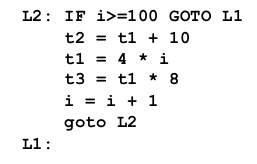
\includegraphics[width=0.3\textwidth]{p80.png}
         \caption{i is abasic induction variable, t1 t2 are in family ofi, but t2 is not because it violates the condition C2 rule 2.}
         \label{fig:p80}
\end{figure}


\begin{figure}[H]
    \centering
     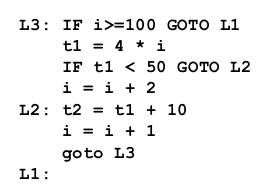
\includegraphics[width=0.3\textwidth]{p81.png}
         \caption{i is abasic induction variable, t1 is in the family of i. t2 is not because it violates the Condition2 rule3(some path reaches t2 includes \texttt{i = i+1} but some not.). }
         \label{fig:p80}
\end{figure}